98. \begin{figure}[ht!]
\center{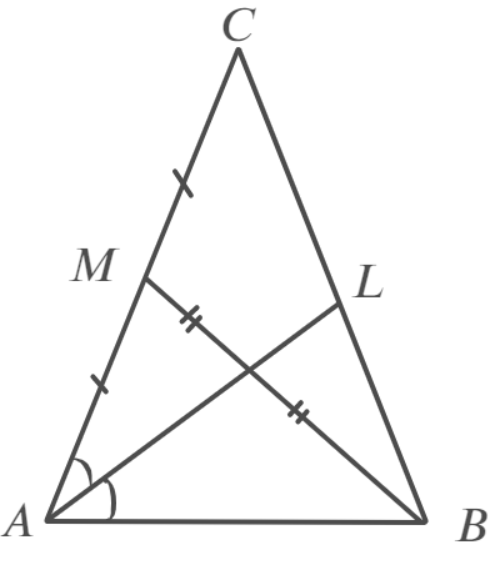
\includegraphics[scale=0.35]{g98.png}}
\end{figure}\\
В треугольнике $AMB$ медиана совпала с биссектрисой, а значит он является равнобедренным и $AB=AM.$ Тогда $AC=BC=2AM=2AB,\ P=AB+AC+BC=5AB=20,\ AB=4,\ AC=BC=8.$\\
